\documentclass[usenames,dvipsnames,notes,11pt,aspectratio=169,hyperref={colorlinks=true, linkcolor=blue}]{beamer}
\usepackage{ifthen}
\usepackage{xcolor}
\usepackage{pgfplots}
\usepackage{amsmath}
\usepackage{centernot}
\usepackage{pifont}
\usepackage{tabularx}
\usepackage{makecell}
\usepackage{cuted}
\usepackage{booktabs}
\usepackage{array}
\usepackage{textcomp}
\usepackage{setspace}
\usepackage{xspace}
\usepackage{subcaption}
\usepackage{tikz}
\usepackage{pdfcomment}
%\newcommand{\pdfnote}[1]{\marginnote{\pdfcomment[icon=note]{#1}}}
\newcommand{\pdfnote}[1]{}

\usepackage{pgfpages}
%\setbeameroption{show notes on second screen}


\input ../beamer-style
\input ../std-macros
\input ../macros

\newcommand{\pt}{\partial}

\AtBeginSection[]
{
    \begin{frame}
        \frametitle{Table of Contents}
        \tableofcontents[currentsection]
    \end{frame}
}
\parskip=10pt

\title[DS-GA.1011]{Tasks and Applications in NLP}
\author[He He]{He He
}
\institute[NYU]{
    
\includegraphics[height=1cm]{../figures/nyu-logo}\\
}
\date{October 4, 2023}

\begin{document}
\begin{frame}
\titlepage
\end{frame}

\begin{frame}
    {Logistics}
    Updates on HW2:\\[1em]
    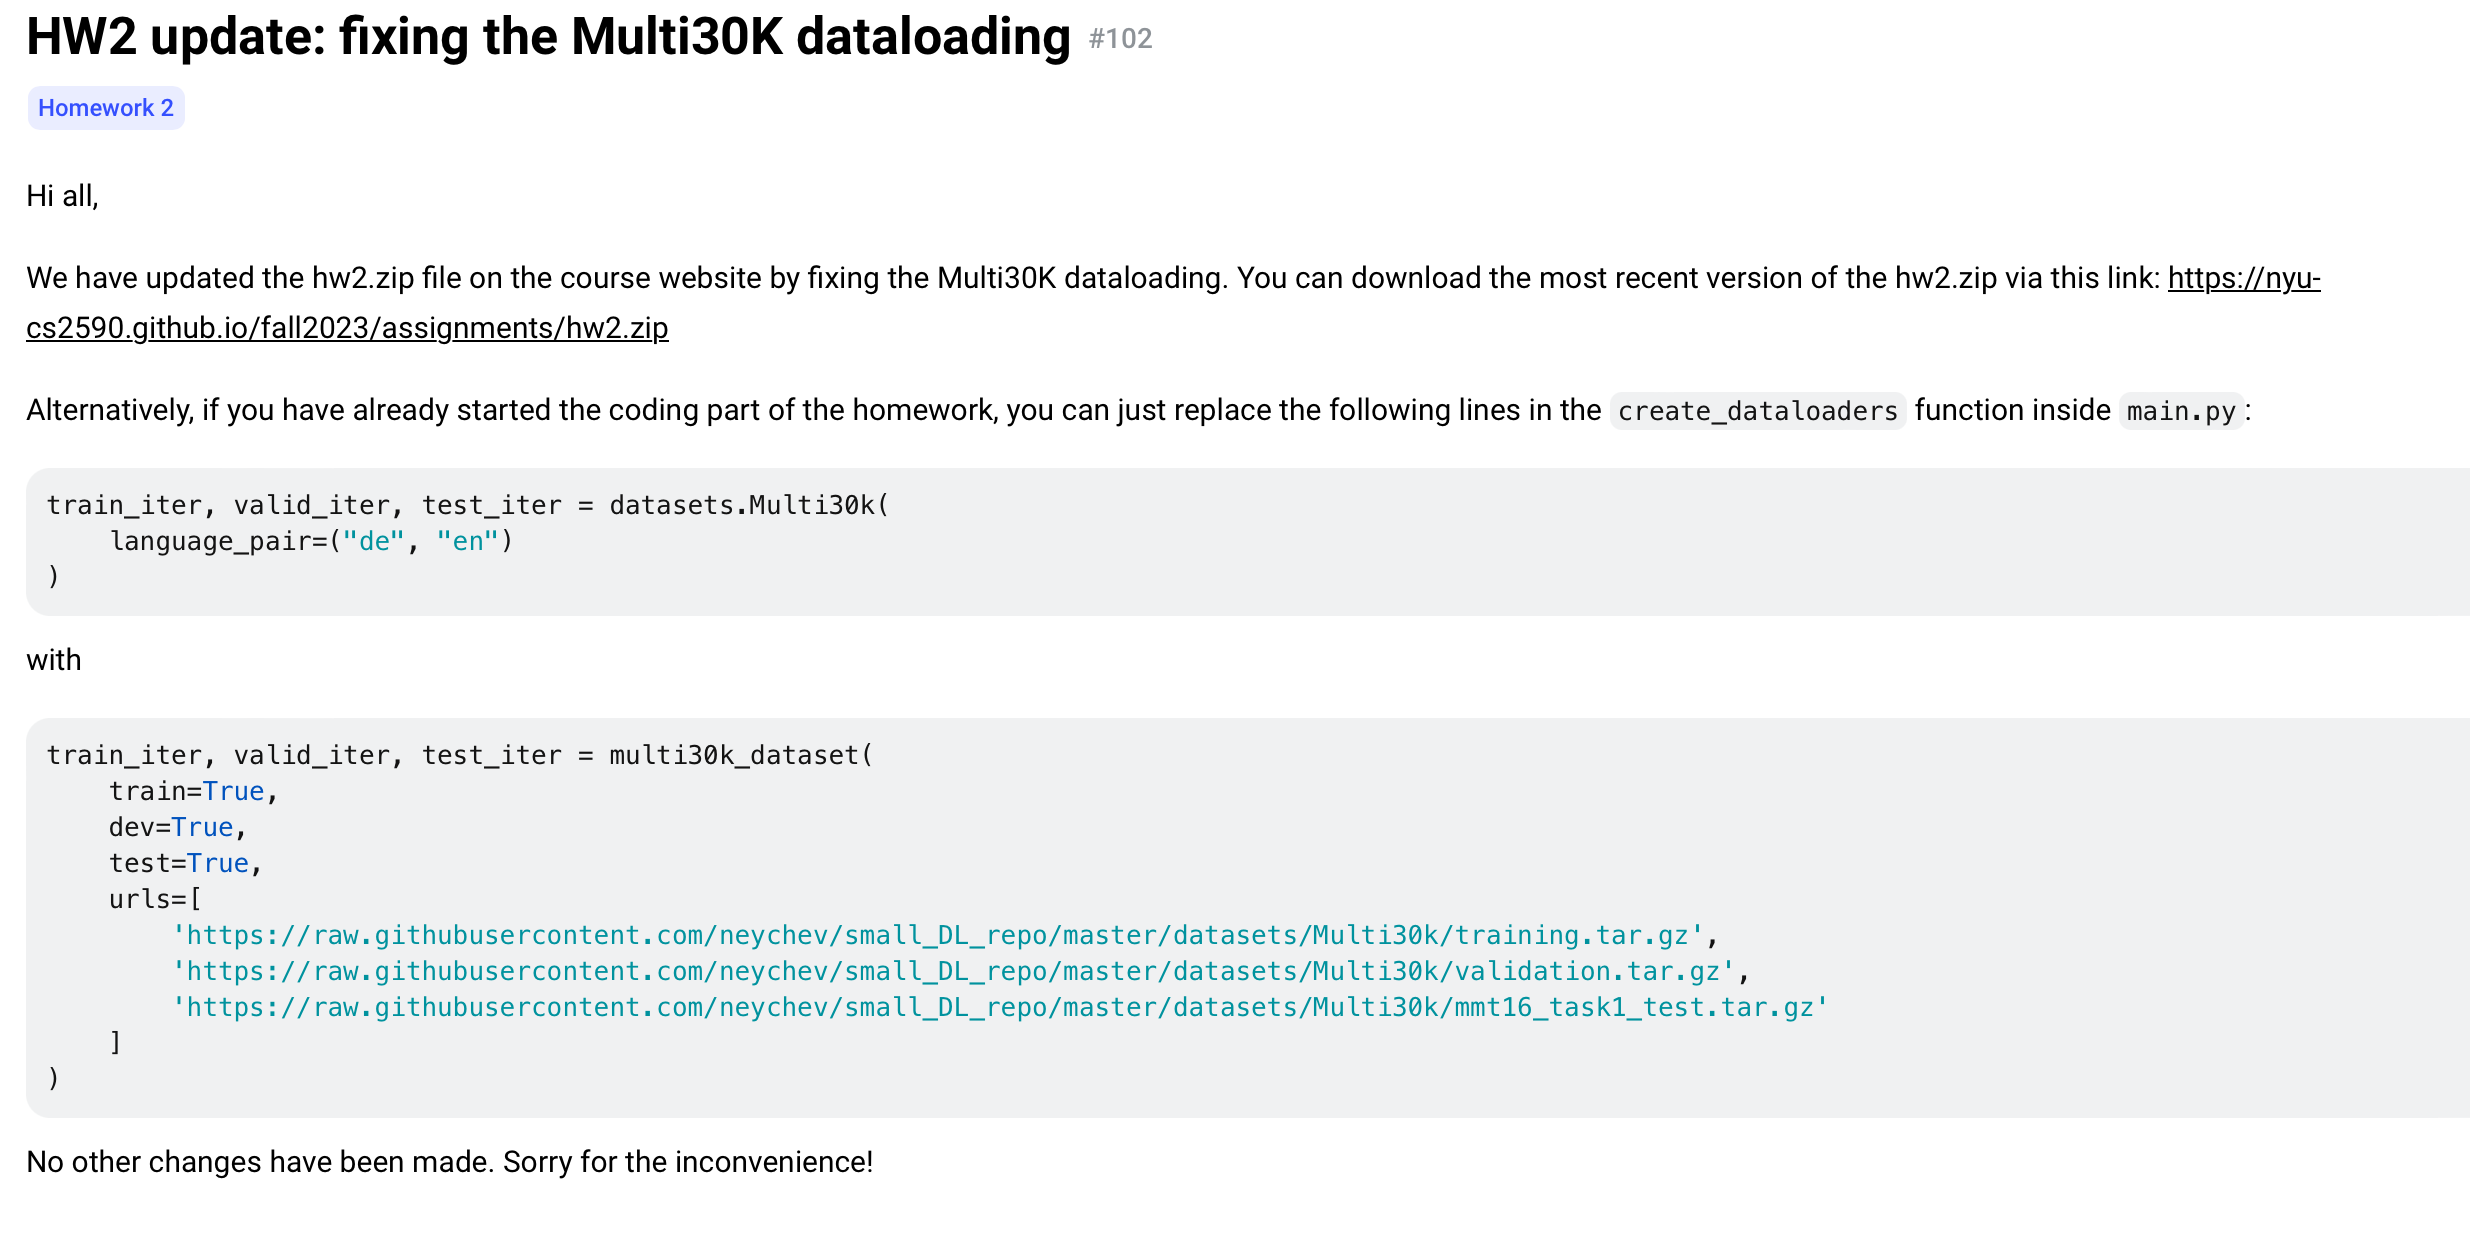
\includegraphics[height=0.7\textheight]{figures/hw2}
\end{frame}

\section{Overview}

\begin{frame}
    {Plan for today}
    \begin{itemize}
        \itemsep1em
        \item So far, we have viewed NLP tasks in a somewhat abstract way (classification, sequence generation).
        \item The actual tasks are much \blue{richer}, each comes with its \blue{unique challenges}.
        \item \textbf{Goal of today}: get a sense of what problems people are working on in NLP and maybe find your own problem!
        \item \textbf{Section}: where to find datasets and how to use them 
    \end{itemize}
\end{frame}

\begin{frame}
    {Two categorizations of tasks}
    By \textbf{purpose}:\\
    \begin{itemize}
        \item \blue{Capabilities}: test key abilities (linguistic, social, cultural, etc.) of language understanding\\
            e.g., parts-of-speech tagging, parsing, commonsense
        \item \blue{Application}: a use case with potential products in mind\\
            e.g., machine translation, question answering
        \item \blue{NLP + X}: new dimensions of capabilities and applications\\
            e.g., multilingual, multimodal
    \end{itemize}

    \pause
    \medskip
    By \textbf{modeling}:\\
    \begin{itemize}
        \item \blue{Classifcation}: output is a categorical variable
        \item \blue{Structured prediction}: output is a chain, a tree, a graph
        \item \blue{Generation}: output is free-form text 
    \end{itemize}
\end{frame}

\section{Capabilities}

\begin{frame}
    {Basic text processing}
    Stanford CoreNLP\vspace{-0cm}
    \begin{figure}
        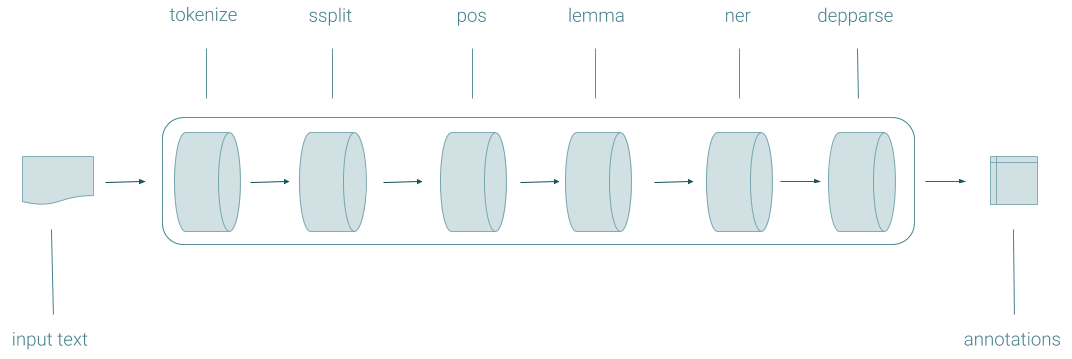
\includegraphics[height=3cm]{figures/pipeline}
        \caption{\url{https://stanfordnlp.github.io/CoreNLP/}}
    \end{figure}\vspace{-0cm}

    \begin{itemize}
        \item Intermediate steps of a pipeline system
        \item Used by downstream models that are more directly connected to an application 
        \item E.g., tokenization $\longrightarrow$ topic models
    \end{itemize}
\end{frame}

\begin{frame}
    {Parts-of-speech tagging}

    Assign each token a part-of-speech tag:
    \begin{figure}
        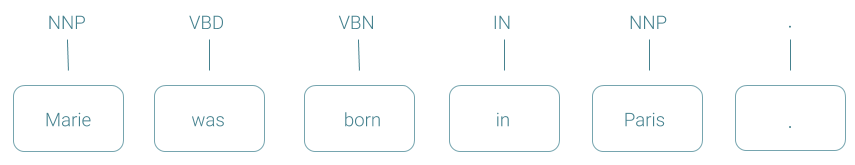
\includegraphics[width=0.8\textwidth]{figures/pos}
        \caption{\url{https://stanfordnlp.github.io/CoreNLP/}}
    \end{figure}

    What is needed to perform this task well?\\\pause
    \begin{itemize}
        \item Memorize possible tags for each word
        \item Model short range context
    \end{itemize}

    What can you do with the output of this task?
    \pdfnote{
        As features of text styles, lemmatization
    }
\end{frame}

\begin{frame}
    {Named entity recognition}

        {\setstretch{1.5}
            $\underbrace{\text{New York University}}_{{\textstyle org}}$ is a private research university based in $\underbrace{\text{New York City}}_{{\textstyle loc}}$.
            It is founded in $\underbrace{\text{1831}}_{{\textstyle year}}$ by $\underbrace{\text{Albert Gallatin}}_{{\textstyle people}}$.\par
            \pause
            $\underbrace{\text{CT of the maxillofacial area}}_{{\textstyle test}}$ showed no facial $\underbrace{\text{bone fracture}}_{{\textstyle symptom}}$.\par
            %$\underbrace{\text{CT of the brain}}_{{\textstyle test}}$ showed no acute changes.\par
        }

        What is the challenge in this task?\\\pause
        \begin{itemize}
            \item Variations of references to an entity (NYU, New York Uni)
            \item Ambiguity (Washington: state or people?)
                \begin{itemize}
            \item Related task: entity linking (multiple people can be named Washington)
                \end{itemize}
        \end{itemize}

        \pause\medskip
        Useful for information extraction or knowledge base construction
\end{frame}

\begin{frame}
    {Parsing}

        \textbf{Syntactic structures} of a sentence:\\
            \begin{itemize}
                \item {\bf Constituents}: small components in a sentence that \blue{compose} into larger ones\\[1ex]
                    \begin{tikzpicture}
                        \node (a) {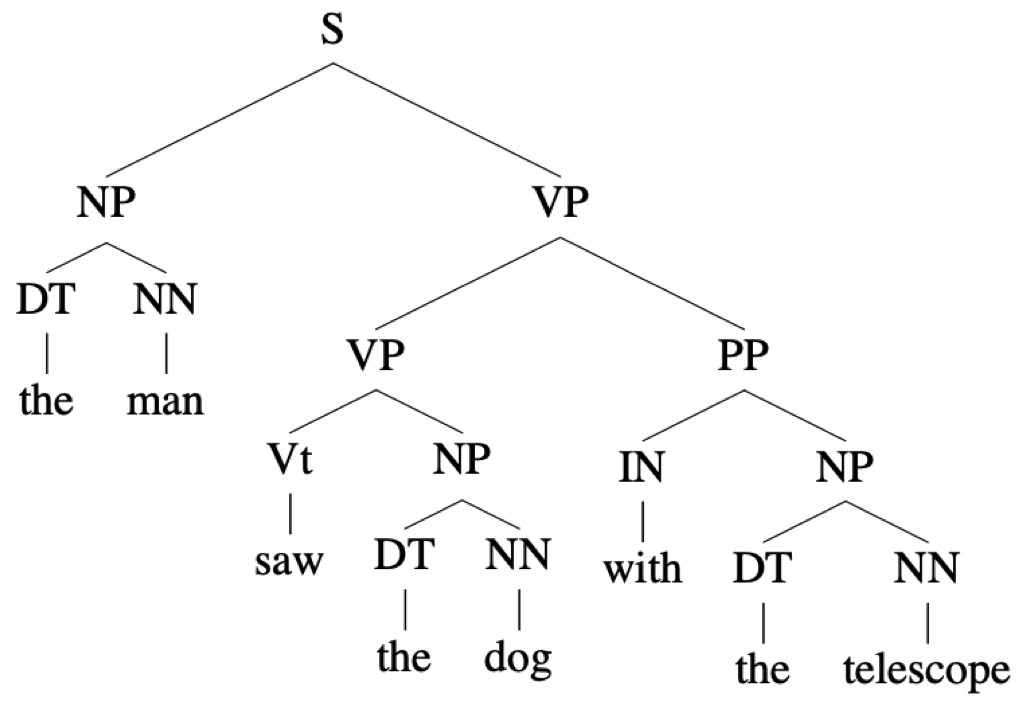
\includegraphics[height=3cm]{figures/parse-tree}};
                        \node [right= of a] {context free grammars};
                    \end{tikzpicture}
                \pause
            \item {\bf Dependencies}: \blue{relations} between words (modify, arguments of etc.)\\[1ex]
                    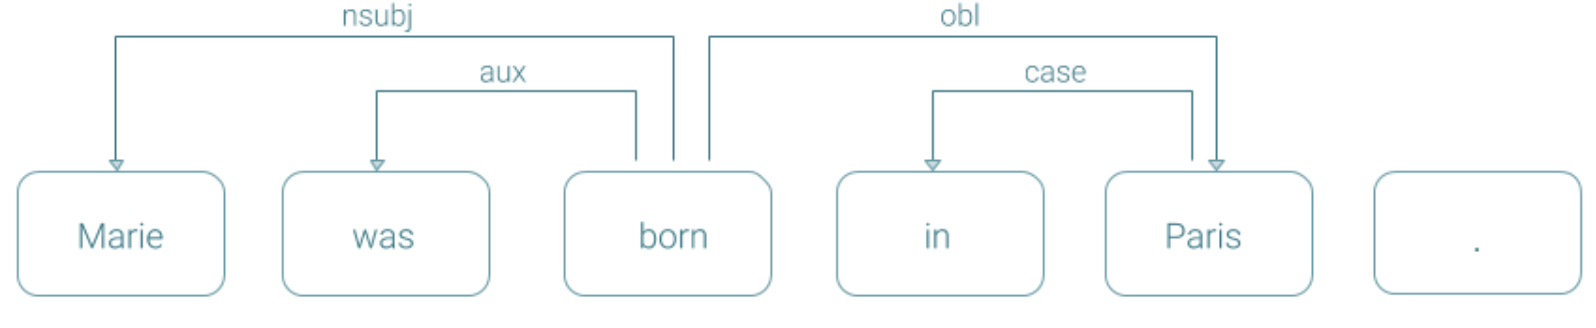
\includegraphics[width=0.7\textwidth]{figures/dep-parse}
            \end{itemize}
\end{frame}

\begin{frame}
    {Parsing}
    What are the challenges?\\\pause
    \begin{itemize}
        \item Design and annotate sentences with parse trees 
        \item Parsing algorithm: find the highest scoring tree out of all possible trees
        \item Multilingual support
    \end{itemize}

    \pause\bigskip
    Why do we need parsing?\\
    \begin{itemize}
        \item A model that understands a sentence must understand its structure (even if not explicitly)
        \item More generally, it's a study about compositionality (which is key to language understanding).
    \end{itemize}
\end{frame}

\begin{frame}
    {Coreference resolution}

    \blue{John} had a great evening meeting with \blue{his} high school friends.\par

    What are the challenges?\\\pause
    \begin{itemize}
        \item Sometimes there're surface cues, othertimes it requires semantic understanding\\
            \href{https://nlp.cs.berkeley.edu/pubs/Durrett-Klein_2013_Coreference_paper.pdf}{Easy Victories and Uphill Battles in Coreference Resolution} \mycite{Durret and Klein, 2013}
        \item Commonsense reasoning (Winograd schema challenge)\\\medskip
            The \green{city councilmen} refused the \red{demonstrators} a permit because \green{they} feared violence.\par
    \end{itemize}
\end{frame}

\begin{frame}
    {Commonsense reasoning}

    \textbf{Motivation}: many tasks requires commonsense knowledge. Can we construct a separate test for it?\pause

    \bigskip
    Which one is the most likely continuation? (example from Hellaswag \mycite[https://arxiv.org/abs/1905.07830]{Zellers et al., 2019})

    A woman is outside with a bucket and a dog. The dog is running around trying to avoid a bath. She...\\
    \begin{itemize}
        \item[A] rinses the bucket off with soap and blow dry the dog’s head.
        \item[B] uses a hose to keep it from getting soapy.
        \item[C] gets the dog wet, then it runs away again.
        \item[D] gets into a bath tub with the dog.
    \end{itemize}
    \pdfnote{C}
\end{frame}

\section{Applications}

\begin{frame}
    {Toxicity classification}

    \begin{tabular}{ll}
        The profoundly stupid have spoken. & \red{toxic}\\
        The president makes himself an easy target. & \green{okay}
    \end{tabular}

    \pause\bigskip
    What is the use case?\pause \hspace{2cm} content moderation

    \bigskip
    What are the challenges?\\\pause
    \begin{itemize}
        \item Toxicity may need to be interpreted in context \mycite{Pavlopoulos et al., 2020}
            \begin{itemize}
                \item[-] \onslide<6->{Hmmm. The flame on top of the gay pride emblem can probably be interpreted in a manner that I did not consider. Perhaps one icon on each end using?}
                \item[-] \onslide<5->{Hi Gadget, interpreted in what manner? \red{Flaming gays? Or Burn a gay?}}
            \end{itemize}
            \onslide<7->{
            \item Dataset biases (section)}
    \end{itemize}
\end{frame}

\begin{frame}
    {Question answering}

    \begin{columns}
        \begin{column}{0.5\textwidth}
            \begin{figure}
                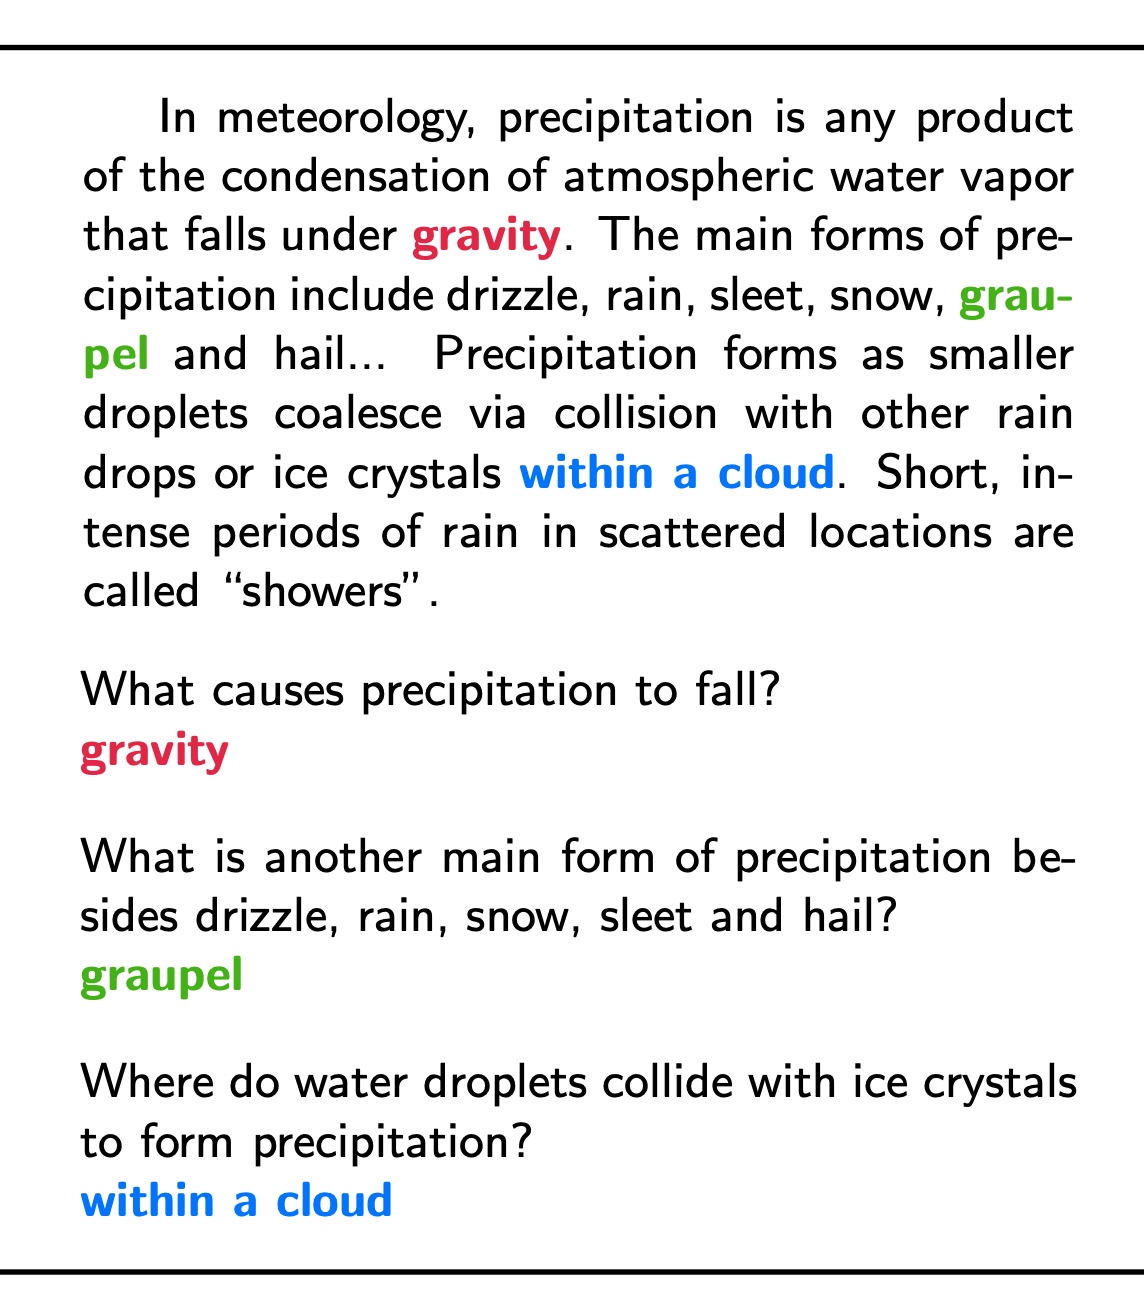
\includegraphics[height=0.7\textheight]{figures/squad}
                \caption{\href{https://arxiv.org/pdf/1606.05250.pdf}{SQuAD}}
            \end{figure}
        \end{column}
        \begin{column}{0.5\textwidth}
            \textbf{Reading comprehension} (close-book QA):\\
            \begin{itemize}
                \item[] Input: document and question
                \item[] Output: start and end indices of the answer span
            \end{itemize}

            \bigskip
            What are the challenges?\\
            \begin{itemize}
                \item Long documents (see \href{https://arxiv.org/abs/2112.08608}{long text QA})
                \item Unanswerable questions (see \href{https://arxiv.org/abs/1806.03822}{SQuAD 2.0})
            \end{itemize}
        \end{column}
    \end{columns}
\end{frame}

\begin{frame}
    {Question answering}
    \begin{columns}
        \begin{column}{0.5\textwidth}
            \begin{figure}
                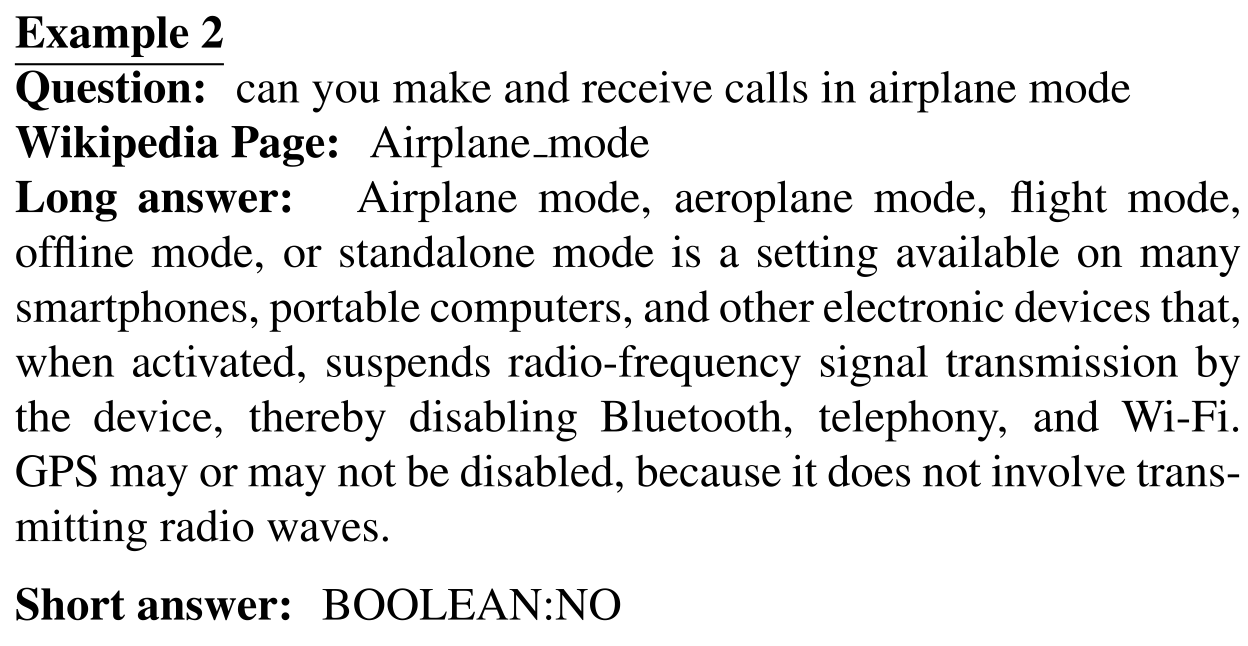
\includegraphics[height=0.5\textwidth]{figures/nq}
                \caption{\href{https://aclanthology.org/Q19-1026.pdf}{Natural questions}}
            \end{figure}
        \end{column}
        \begin{column}{0.5\textwidth}
            \textbf{Open-domain question answering}:\\
            \begin{itemize}
                \item[] Input: question
                \item[] Output: answer (in text)
            \end{itemize}

            \bigskip
            What are the challenges?\\
            \begin{itemize}
                \item Retrieval
                \item Evaluation (see \href{https://arxiv.org/abs/2109.05289}{equivalent answers})
                \item Presupposition (see \href{https://aclanthology.org/2021.acl-long.304.pdf}{Kim et al., 2021})\\
                    What is the stock symbol for mars candy?
                    \pdfnote{mars is not a publicly traded company}
            \end{itemize}
        \end{column}
    \end{columns}
\end{frame}

\begin{frame}
    {Summarization}
    \begin{columns}
        \begin{column}{0.5\textwidth}
            \begin{figure}
                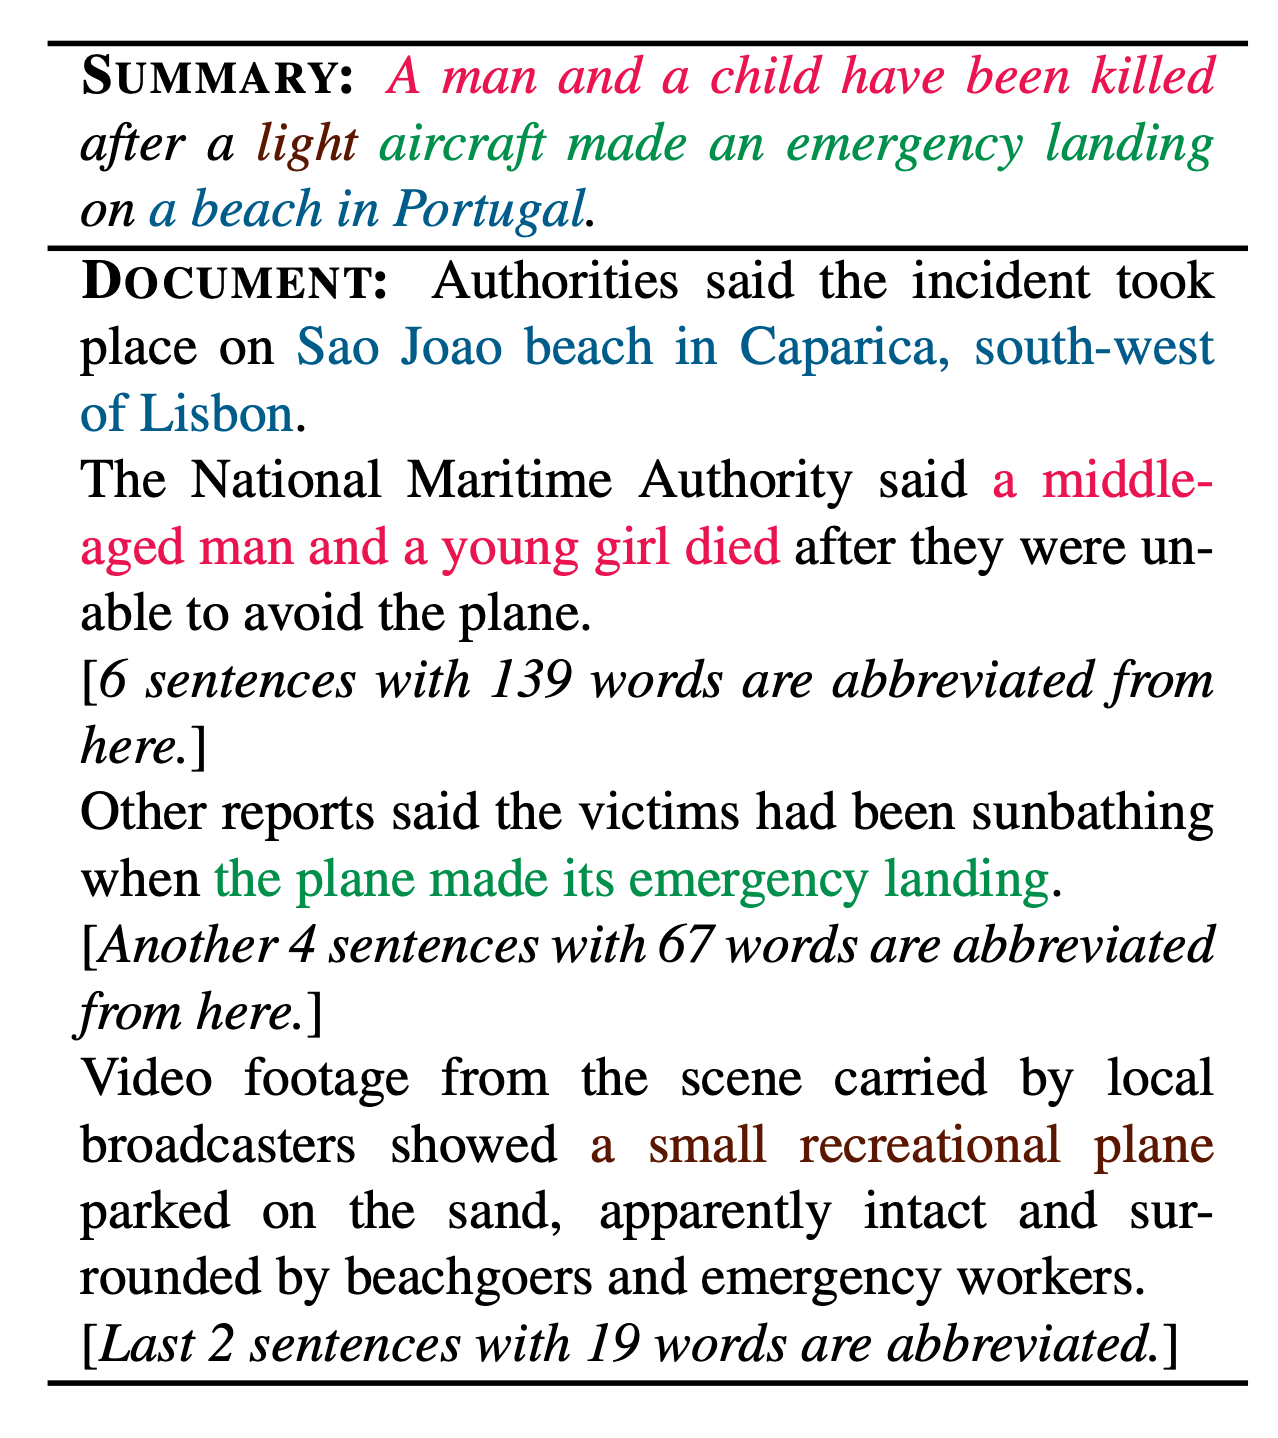
\includegraphics[height=0.8\textwidth]{figures/xsum}
                \caption{\href{https://aclanthology.org/D18-1206.pdf}{XSum}}
            \end{figure}
        \end{column}
        \begin{column}{0.5\textwidth}
            \textbf{Abstractive summarization}:\\
            \begin{itemize}
                \item[] Input: document (e.g., a news article)
                \item[] Output: summary (in text)
            \end{itemize}
            
            \medskip
            \textbf{Extractive summarization}:\\
            \begin{itemize}
                \item[] Input: document 
                \item[] Output: $k$ sentences from the document 
            \end{itemize}

            \bigskip
            What are the challenges?\\
            \begin{itemize}
                \item Evaluation: what is a good summary?
                \item Faithfulness (see \href{https://arxiv.org/abs/2005.03754}{Durmus et al., 2020})
            \end{itemize}
        \end{column}
    \end{columns}
\end{frame}

\begin{frame}
    {Semantic parsing}

    Natural language to formal language:\\
    \begin{itemize}
        \item Input: text (e.g., question, instruction)
        \item Output: logical form (DSL, e.g., SQL) $\longrightarrow$ execute to get result
    \end{itemize}

    \begin{figure}
        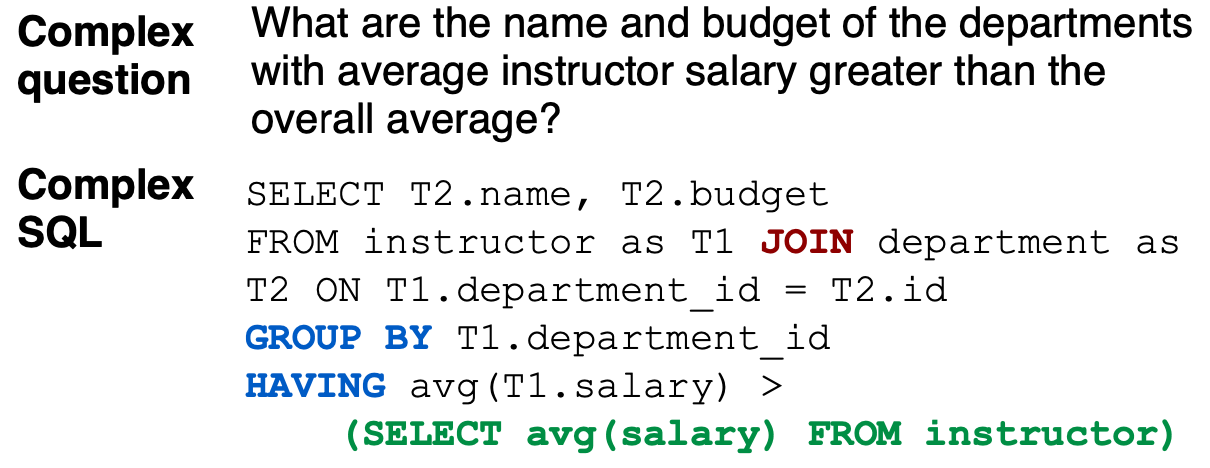
\includegraphics[height=3cm]{figures/text2sql}
        \caption{\href{https://arxiv.org/pdf/1809.08887.pdf}{Spider}}
    \end{figure}

    What are the use cases?\\
    \begin{itemize}
        \item Interface with a database, interpreter (shell, python)
        \item More generally, interact with a computer
    \end{itemize}
\end{frame}

\begin{frame}
    {Categorization of tasks by modeling}

    \textbf{Classification}: text $\rightarrow$ $\pc{1,\ldots,K}$\\
    \begin{itemize}
        \item E.g., Toxic classification, natural language inference, multiple choice QA
    \end{itemize}

    \textbf{Structured prediction}: \\
    \begin{itemize}
        \item Sequence labeling: $\sV_{\text{in}}^n \rightarrow \sV_{\text{out}}^n$
            \begin{itemize}
                \item E.g., POS tagging, NER (using the BIO annotation), close-book QA 
            \end{itemize}
        \item Parsing: $\sV_{\text{in}}^n \rightarrow \text{tree}$
                \begin{itemize}
                    \item E.g., constituent, dependency, semantic parsing 
                \end{itemize}
    \end{itemize}
\end{frame}

\begin{frame}
    {Categorization of tasks by modeling}

    \textbf{Generation}: $\sV_{\text{in}}^n \rightarrow \sV_{\text{out}}^m$\\
    \begin{itemize}
        \item Classification: $m=0, \sV_{\text{out}}=\pc{1,\ldots,K}$
        \item Structured prediction with linearized annotation\\[1ex]
            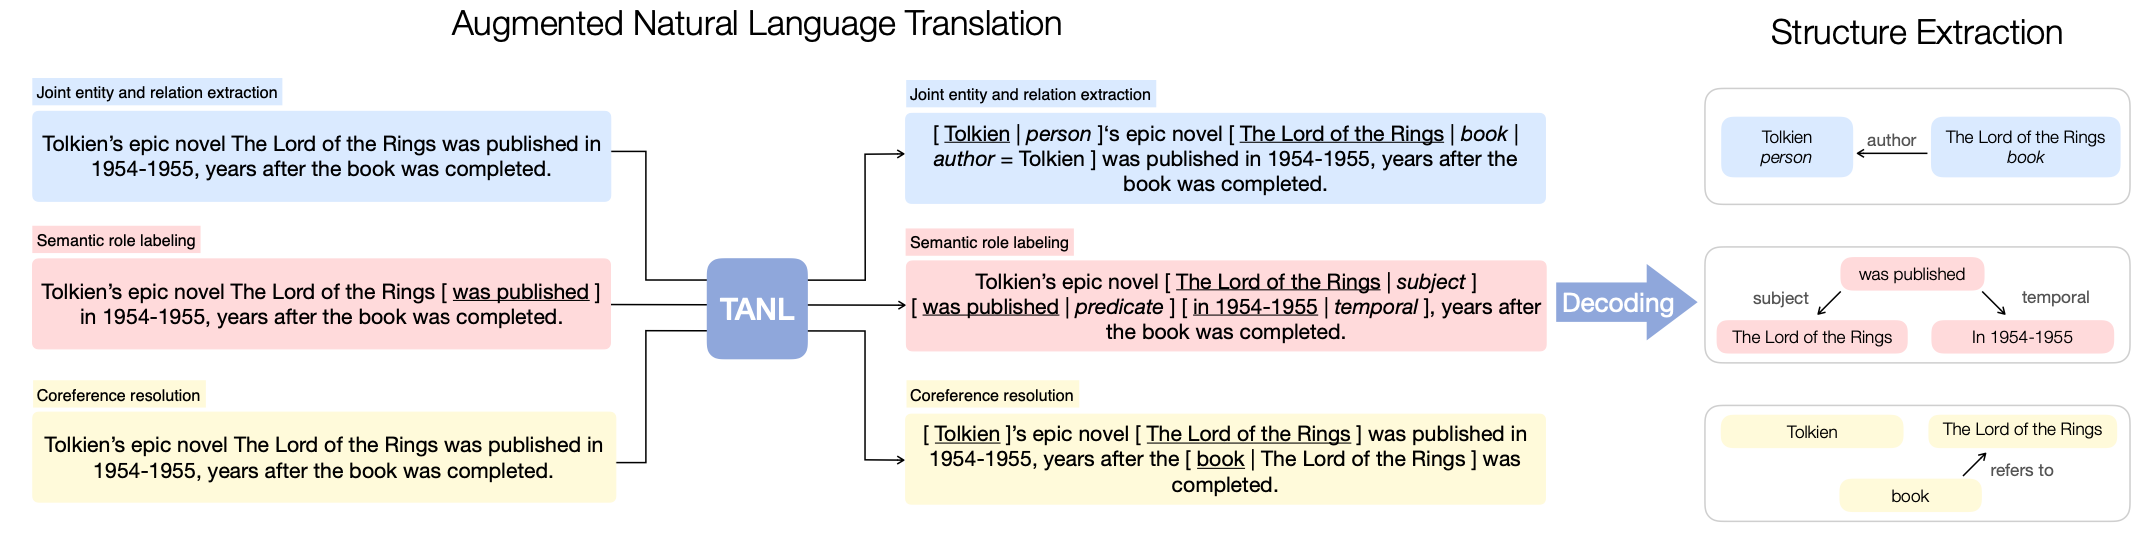
\includegraphics[height=3cm]{figures/tanl}
        \item Sequence to sequence, e.g., machine translation, summarization, text-to-code
    \end{itemize}

    The most general format (pros and cons?)
\end{frame}

\section{Evaluation}

\begin{frame}
    {Structured prediction}

    \textbf{Exact match}: unit of comparison is the whole structure\\
    \begin{itemize}
        \item \blue{output} is correct only if it is exactly the same as the \blue{reference}
    \end{itemize}

    \pause
    How do we account for partial correct answers?

    \textbf{F1}: unit of comparison is components of the structure\\
    \begin{itemize}
        \item Define components of the output
        \item Compute overlap of \blue{components} in terms of F1 between each predicted structure and its reference 
        \item Average the F1 score over all examples
    \end{itemize}
    \pause

    Example: reading comprehension\\
    \begin{itemize}
        \item predicted = skilled workers = \pc{\text{skilled}, \text{workers}}
        \item reference = an increase in skilled workers = \pc{\text{skilled}, \text{workers}, \text{an}, \text{increase}, \text{in}}
        \item precision =
        \item recall =
    \end{itemize}
\end{frame}

\begin{frame}
    {Generation}

    \textbf{Task}: given the reference(s) of each source sentence, evaluate the quality of the generated sequences.
    \begin{description}
        \item[Reference 1] It is a guide to action that ensures that the military will forever heed Party commands.
        \item[Reference 2] It is the guiding principle which guarantees the military forces always being under the command of the Party. 
        \item[Candidate 1] It is a guide to action which ensures that the military always obeys the commands of the party.
        \item[Candidate 2] It is to insure the troops forever hearing the activity guidebook that party direct.
    \end{description}

    \pause
    \textbf{Main idea}: good generations should have high overlap with the reference.
\end{frame}

\begin{frame}
    {BLEU: n-gram precision}
    \textbf{First try}: n-gram precision ($x$: input, $c$: candidate, $r$: references)
    $$
    p_n = \frac{
        \sum_{(x,c,r)} \sum_{s\in\text{n-gram}(c)} \BI\pb{s \text{ in } r}
    }
    {
\sum_{(x,c,r)} \sum_{s\in\text{n-gram}(c)} \BI\pb{s \text{ in } c}
    } = \frac{
        \text{\# n-grams in both cand and ref}
    }{
        \text{\# n-grams in cand}
    }
    $$
    \pause
    \textbf{Problem}: can match only a few words in the reference(s)\\
    \begin{description}
        \item[Candidate] the the the the the the the
        \item[Reference 1] The cat is on the mat
        \item[Reference 2] There is a cat on the mat
    \end{description}
    unigram precision = ?

    \textbf{Solution}: clip counts to maximum count in the reference(s)
\end{frame}

\begin{frame}
    {BLEU: combine n-gram precision}

    Compute n-gram precision for each $n$ (typically up to 4)

    Then, we need to combine the n-gram precisions.

    Average? Problem: precision decreases roughly exponentially with $n$.

    \pause
    \textbf{Solution}: geometric mean (when $w_n=1/n$)
    $$
    \exp\p{\sum_{i=1}^n w_n \log p_n}
    $$
\end{frame}

\begin{frame}
    {BLEU: brevity penalty}

    Problem with precision: ``One who does nothing also does nothing wrong''

    \begin{description}
        \item[Candidate] of the 
        \item[Reference 1] It is the guiding principle which guarantees the military forces always being under the command of the Party. 
        \item[Reference 2] It is the practical guide for the army always to heed the directions of the party.
    \end{description}

    Why not use recall? %with \textit{multiple} references?
    \pdfnote{
       BLEU does not use recall because the notion of recall is unclear when simultaneously matching against multiple reference translations (rather than a single reference).  
    }
\end{frame}

\begin{frame}
    {BLEU: brevity penalty}

    %A good translation must match the reference in:\\
    %\begin{description}
    %    \item[word choice] captured by precision
    %    \item[word order] capture by n-gram
    %    \item[length] ?
    %\end{description}

    \textbf{candidate length} $C=\sum_{(x,c,r)} \text{len}(c)$

    \textbf{reference length} $R=\sum_{(x,c,r)} \argmin_{a\in\pc{\text{len}(r_1),\ldots,\text{len}(r_k)}} |a-\text{len}(c)|$\\
    \begin{itemize}
        \item Use the reference whose length is closest to the candidate
    \end{itemize}

    \textbf{Brevity penalty} $BP =
    \begin{cases}
        1 & \text{if } c \ge r \quad \text{no penalty}\\
        e^{1-R/C} & \text{if } c < r \quad \text{downweight score}
    \end{cases}
    $
\end{frame}

\begin{frame}
    {BLEU}
    Putting everything together:
    \begin{align*}
        \text{BLEU} &= BP\cdot \exp\p{\sum_{n=1}^N w_n \log p_n} \\
        %\log \text{BLEU} &= \min(1-\frac{R}{C}, 0) + \sum_{n=1}^N w_n \log p_n
    \end{align*}
    \vspace{-2em}

    \pause
    A good translation should match the references in word choice, word order, and length. (How is each part captured by BLEU?)

    \pause
    Practicalitis:\\
    \begin{itemize}
        \item Both precision and the brevity penalty are computed at the \emph{corpus level}.
        \item Need smoothing for sentence-level BLEU.
        \item Good correlation with human evaluation for MT (typically $n=4$).
    \end{itemize}
\end{frame}

\begin{frame}
    {ROUGE}
    \textbf{Task}: given a candidate summary and a set of reference summaries, evaluate the quality of the candidate.

    \textbf{ROUGE-n}: n-gram recall\\
    \begin{itemize}
        \item Encourage content coverage 
    \end{itemize}

    \textbf{ROUGE-L}: measures longest common subsequence between a candidate and a reference (doesn't require consecutive match.)\\
    \begin{itemize}
        \item Precision $ = LCS(c, r) / \text{len}(c)$
        \item Recall $ = LCS(c, r) / \text{len}(r)$
        \item F-measure $ = \frac{(1+\beta^2)RR}{R + \beta^2 P}$
    \end{itemize}
\end{frame}

\begin{frame}
    {Automatic evaluation metrics for generation}
    n-gram matching metrics (e.g. BLEU, ROUGE)\\
    \begin{itemize}
        \item Measures exact match with reference; interpretable.
        \item Do not consider semantics.
    \end{itemize}

    Embedding-based metrics (e.g. BERTScore, MAUVE)\\
    \begin{itemize}
        \item Measures similarity to the reference in an embedding space.
        \item Captures synonyms and simple paraphrases.
    \end{itemize}

    However, we also want to measure\\
    \begin{itemize}
        \item Is the generation correct? e.g. faithfulness (summarization), adequacy (MT).
        \item Open-ended generation: is the story/dialogue interesting, informative, engaging?
        \item So \textbf{human evaluation} is still needed.
    \end{itemize}
\end{frame}

%\section{NLP + X}
%
%\section{Where does the data come from?}
%
%\begin{frame}
%    {Synthetic data}
%\end{frame}

\section{Final projects}

\begin{frame}
    {Common types of projects}
    \textbf{Find a nail}: identify a \blue{problem/domain} that you are excited about and try to solve it using whatever method that works

    %Example:\\
    \begin{tikzpicture}
        \node (a) {
\includegraphics[height=3cm]{figures/proj-1}};
        \node (b) [right=0cm of a] {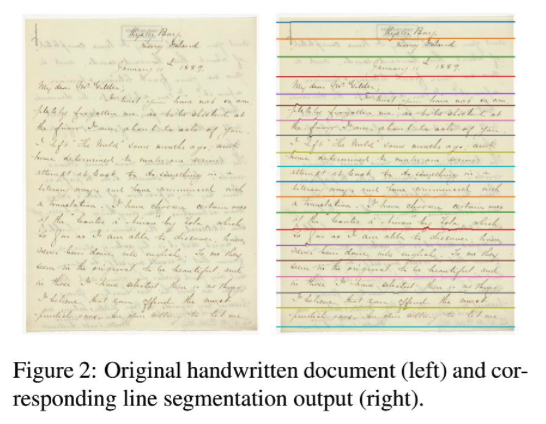
\includegraphics[height=3cm]{figures/proj-1-1}};
    \end{tikzpicture}

    Likely to succeed if:\\
    \begin{itemize}
        \item You know a domain and its challenges very well
        \item You have access to (high-quality, large) data (\blue{important!})
        \item You have a reliable way to evaluate the result
    \end{itemize}
\end{frame}

\begin{frame}
    {Common types of projects}
    \textbf{Find a hammer}: identify a \blue{method} that you are excited about and try to improve or extend it on its common use cases 

    %Example:\\
    \begin{tikzpicture}
        \node (a) {
\includegraphics[height=2cm]{figures/proj-2-1}};
        \node (b) [right=0cm of a] {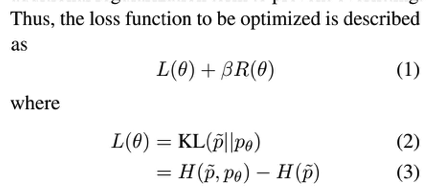
\includegraphics[height=2cm]{figures/proj-2}};
    \end{tikzpicture}

    Likely to succeed if:\\
    \begin{itemize}
        \item You know a method and its variants/extensions well 
        \item You have identified a weakness (e.g., efficiency, reliability, problem-specific challenges) 
    \end{itemize}
\end{frame}

\begin{frame}
    {Common types of projects}
    \textbf{Study a nail or hammer}: \blue{analyze} common methods and their applications 

    %Example:\\
    \begin{tikzpicture}
        \node (a) {
\includegraphics[height=2cm]{figures/proj-3}};
        \node (b) [right=0cm of a] {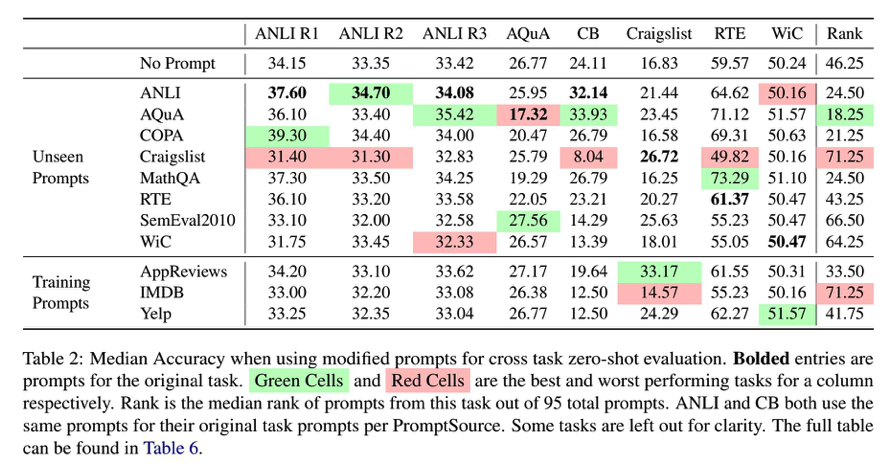
\includegraphics[height=2.5cm]{figures/proj-3-1}};
    \end{tikzpicture}

    Likely to succeed if:\\
    \begin{itemize}
        \item You have an interesting question to ask 
        \item You are good at running large scale experiments 
    \end{itemize}
\end{frame}

\begin{frame}
    {Project proposal}
    Before submitting the proposal:\\
    \begin{itemize}
        \item Form groups and identify a rough topic of interest
        \item Literature survey
        \item Get all resource ready (data, codebase, machines)
    \end{itemize}

    \pause
    Write the proposal:\\
    \begin{itemize}
        \item Overview
            \begin{itemize}
        \item What problem are you going to work on?
        \item What are the challenges?
        \item What's your solution?
            \end{itemize}
        \item Project plan
            \begin{itemize}
                \item What do you plan to do (experiments, data, model)
                \item How do you evaluate success?
            \end{itemize}
    \end{itemize}
\end{frame}

\end{document}
